\subsection{Collecting samples}

The \data{possum} data set is a \term{sample} of the possums in each of the site areas. All of the possums in the areas where traps were set is called the \term{population} of the sample.

Ideally, any ``citizen'' of the population can be sampled. In the \data{possum} data set, this means that any possum in the population of all possums in those regions had an actual chance of being included in the sample.

A jury is an example of the case where not every person in the population can be sampled. Juries are samples from the population of registered voters. Children (under 18) are certainly not eligible to be in the sample. Former convicts also are not sampled to be on jury duty.

When making any conclusions

The population that is the source of the sample is the 


Ideally, sampling is 

Usually this sampling is random or assumed to be random.

%Given the sample, it would be nice to make conclusions about possums in general and not just about those possums in the sample. For instance, if the sample shows a drastic difference in gender ratio (number of males to females) between possums between the two possible \var{Pop} values, then it would be important if this meant the populations also had a difference.

%First and foremost, a sample is only guaranteed to say something about the population it came from. Possums are also found in New Guinea, however, since the possums in the sample are not from this island, nothing conclusive can be said about New Guinea possums. On the other hand, if it is reasonable to say the possums in the sample is made from all of possums in Victoria, New South Wales, and Queensland, then the sample can be used to make conclusions about possums in these areas. It is always possible to make an assumption that the possums in the sampled areas and the possums of New Guinea are basically the same, however, this assumption may or may not be reasonable since there is no data to support it. This means any conclusions made about the New Guinea possums from the \data{possum} data set hinge upon the accuracy of this assumption.
\begin{center}
\vspace{0.5cm}

Graphic displaying sampling of population in subset of Australia and its relation to New Guinea.

\vspace{0.5cm}
\end{center}

Often times, \emph{some} assumptions are needed. For instance, a statistician might assume a possum's chance of being trapped is not dependent on its gender. The point to take away from this discussion on making assumptions is not to abandon them altogether but to suggest caution when making assumptions. And when assumptions are made, they should be identified, understood, and expressed when making conclusions.

What really is important to ask with a data set is, what population does this data really represent? From here, assumptions are needed to extend conclusions to larger populations.

\subsection{Bias, error, and uncertainty}

\subsubsection{Identifying the population}

Which would you trust more: a poll where the people were randomly selected to take part or one where people searched out the poll to participate? Most polls reported in the media are of the first type while many polls on the internet are of the second type. Of the second, this is called a \term{convenience sample}, and these are generally not representative of the general population.

Ideally, a sample is selected randomly from the population that is representative. Individuals from every corner of the population at least have a chance of being included in the sample. This isn't always the case. If an internet poll, the only population that might be included are those of internet users.
\begin{center}
   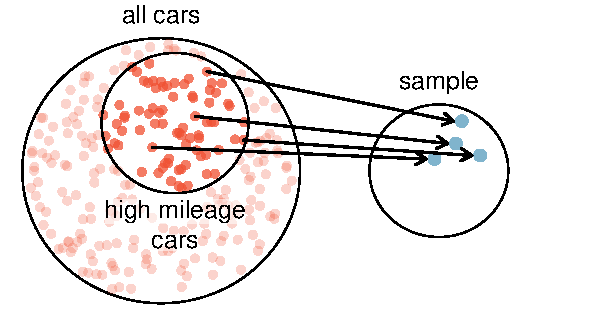
\includegraphics[height=1.6in]{ch1/popToSample/popToSubSample}
\end{center}
If the website had a political leaning, such as the liberal Huffington Post or the conservative CNS News' site, then an even smaller section of the population will be included that is rarely representative of the opinions of the population as a whole.
\begin{center}
   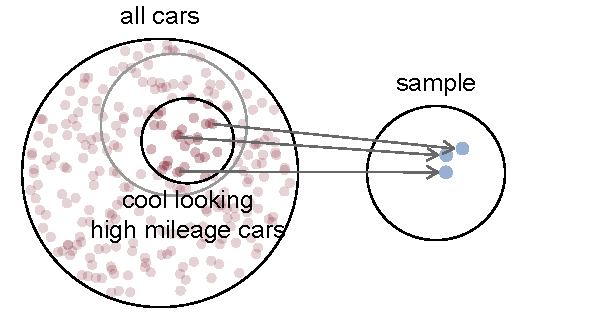
\includegraphics[height=1.6in]{ch1/popToSample/popToSubSubSample}
\end{center}
%Even if the information from the sample did represent the entire popul
%The tragedy is that, in practice, these polls are generally so skewed to one sector of the population that no matter how many corrections are made the data is nearly useless.
%For example, would a poll on the approval rating of Barack Obama produce similar results on Huffington Post's website and CNS News' site? Since one tends to show favor to the political left and the other the political right, really different populations are likely to respond. At best, such a poll provides the approval according to Huffington Post or CNS News readers\footnote{At worst, it provides the approval according to a small number of individuals who are computer-saavy enough to vote many times.}.
Convenience sampling usually invokes a \term{bias} into the data that can usually not be corrected.
%\begin{center}
%\vspace{1.5cm}
%Graphic showing sampling of different parts of the population. \\
%No caption needed.
%\vspace{1.5cm}
%\end{center}

\subsubsection{Randomness}

Another difficulty in sampling is \term{self-selection bias}; individuals who participate must agree to do so. Granted, freedoms are certainly a good thing but the difficulties in sampling that arise from those freedoms are a nuisance when analyzing data, making interpretations of the data more difficult.

One 

In addition to sampling the from the entire population, one of the most important components of sampling is selecting individuals from that population randomly. Another downfall of internet polls or any convenience sample is a \term{self-selection bias}; any individual in the sample actively choose to be in the sample.

%While people cannot be forced to participate, the animals captured in the \data{possum} data set had no such choice.

Polls where the people polled are randomly selected from the population are more dependable for a specific reason: each person has an opportunity to be included in the sample. In a \term{simple random sample}, each person has an equal opportunity to be included. Most of the samples in this book are assumed to be simple random samples, and when this assumption is not necessarily reasonable it will be mentioned. For instance, it is not guaranteed that the possums are a simple random sample of possums in the sampled regions.
\begin{center}
   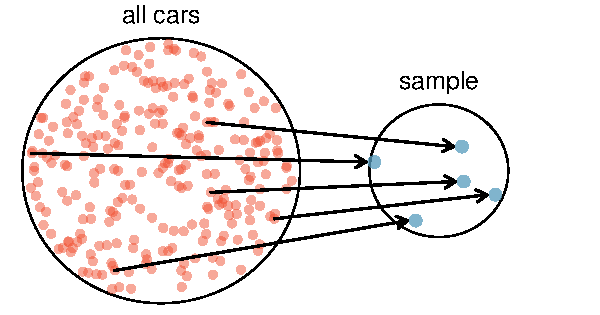
\includegraphics[height=1.6in]{ch1/popToSample/popToSample}
\end{center}


\subsubsection{Systematic bias}

\begin{example}{Suppose after measuring all of the possum lengths, the researchers realized their measuring stick had been shaved off at the bottom 1cm. How would this affect the measurements of the variable \var{totalL}?}
The first possum was measured at 89cm. In this case, since the measuring stick inflated the length by 1cm so this possum's true length would be 88cm. This inflated length would be true of all possums, so to the possums' measured lengths would be 1cm too long.
\end{example}

If this had occurred with the measurements of \var{totalL}, then these measurements represent another form of bias called a \term{systematic biased} because they are not accurately assessing the actual length. In some cases, such as this one, a systematic bias can be corrected.

\subsubsection{Measurement error}

An alternative, and perhaps more likely scenario, is that the measurements are \term{unbiased} but not exact. Observations are never \emph{exact}. If 10 people measured the same possum, they would all probably have slightly different measurements. This variability in the measurements is called \term{measurement error}. Usually this error is assumed to be small relative to the variability from observation to observation (possum to possum, in this case), which permits relatively uncomplicated analyses. If this error is not necessarily small, then this is an important consideration in any analysis of the data.

